\subsection{Motor styring}

På figur \ref{fig:ibd_motorcontrol} vises det interne blok diagram for motor control blokken. Blokken består af 4 ESC'er, 4 motorer og et 12V batteri. 12V batteriet står for forsyning til hele blokkken, mens de PWM signaler der sendes ind i ESC'erne bestemmer hvor meget forsyning motorerne tildeles. Den PWM der sendes til ESC'er sendes med en duty cycle mellem 40-80\%. Ved ændring af duty cyclen, ændres forsyningen til dronens motorer. Ved en ændring af forsyning ændres hastigheden hvorved motorerne drejer  med.

\begin{figure}[H]
\centering
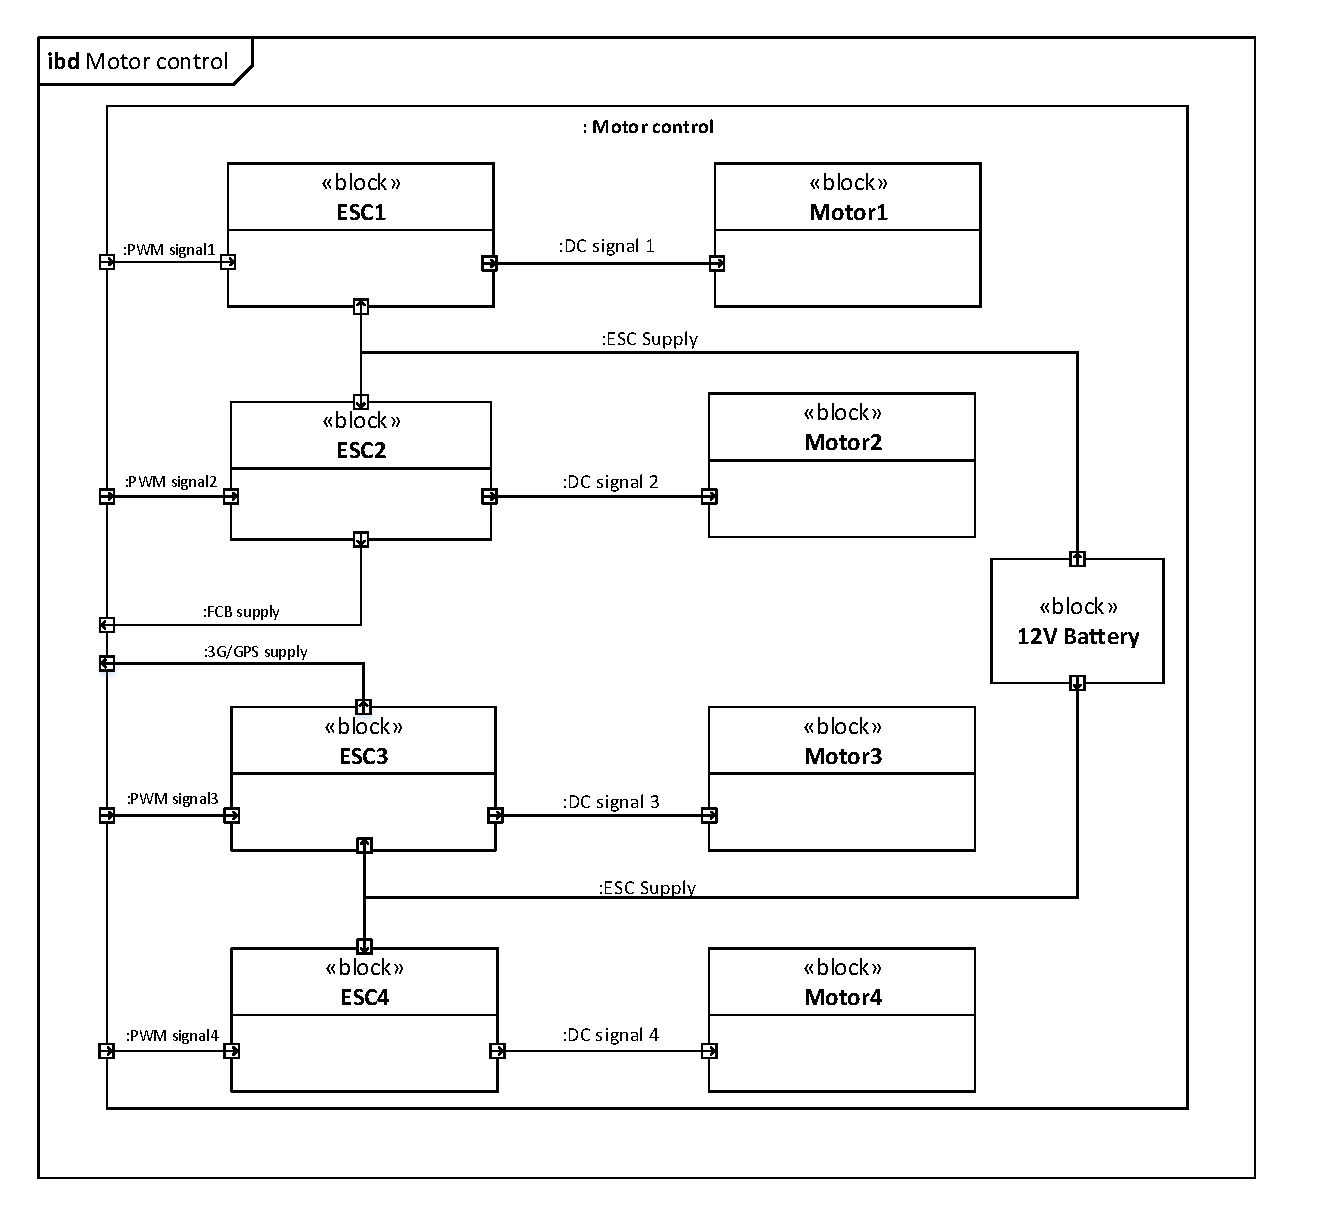
\includegraphics[width=1\textwidth]{Billeder/IBD/ibd6_motorcontrol.pdf}
\vspace{-1cm}
\caption{Ibd - Motor control}
\label{fig:ibd_motorcontrol}
\end{figure}

\begin{table}[H]
	\centering
		\begin{tabular}{|p{2.5 cm}|p{5.5 cm}|p{2.5 cm}|p{2.5 cm}|} 
		\hline
			\textbf{Signal navn} 	& \textbf{Signal beskrivelse}		& \textbf{Out} 				& \textbf{In}     \\ \hline
			PWM signal1 & 400 Hz signal med en duty cycle på 40-80 $\%$ & Flight control board. & ESC1.	\\ \hline
			PWM signal2 & 400 Hz signal med en duty cycle på 40-80 $\%$ & Flight control board. & ESC2.	\\ \hline
			PWM signal3 & 400 Hz signal med en duty cycle på 40-80 $\%$ & Flight control board. &	ESC3. \\ \hline
			PWM signal4 & 400 Hz signal med en duty cycle på 40-80 $\%$ & Flight control board. & ESC4. \\ \hline
			DC signal 1 & Et varierende DC. & ESC1. & Motor1.	\\ \hline
			DC signal 2 & Et varierende DC. & ESC2. & Motor2.	\\ \hline
			DC signal 3 & Et varierende DC. & ESC3. & Motor3.	\\ \hline
			DC signal 4 & Et varierende DC. & ESC4. & Motor4.	\\ \hline
			FCB supply & 5V DC. & ESC2 & Flight control board.	\\ \hline
			3G/GPS supply & 5V DC. & ESC3. & 3G/GPS.	\\ \hline
			ESC supply & 12V DC. & Battery. & ESC1/ESC2.	\\ \hline
			ESC supply & 12V DC. & Battery. & ESC3/ESC4.	\\ \hline
			
		\end{tabular}
	\caption{Forbindelser til: Ibd - Motor control}
	\label{tab:IBD_Motor_control}
\end{table}

